\chapter{Introduction}
\label{chapter:introduction}

Neuromorphic computing has developed into a popular scientific field throughout the last years and finds more and more applications and implementations in science and industry, e.g.~\cite{6905473}.
These systems already show advantages over traditional computer architectures, like the von-Neumann architecture, in specific applications and continue to improve.
In its current generation, neural networks abandon discrete time steps and states, but gain more computational power~\cite{Maass19971659}.
They use spikes and continuous time scales that resemble nature more closely and allow for efficient implementations as analog hardware which offers high performance at low energy consumption~\cite{NIPS2015_5862}.
Still, new architectures also require novel styles of programming~\cite{Amir2013CognitiveCP} and users need to adapt to these.
This can be a hurdle for many users when developing new experiments, that initially take a significant amount of time. 
\\
\\
One example for this is the current way of programming for the plasticity processing unit of the \ac{HICANN-DLS}. 
The \ac{HICANN-DLS} is a small scale system that features analog emulation of neurons and synapses in networks~\cite{PPU}.
The \ac{PPU}, as part of \ac{HICANN-DLS}, can be used for implementing plasticity rules in such networks.
It resembles a traditional processor architecture, which was modified for this task.
Implementing such plasticity rules differs from conventional high-level programming styles. 
When creating code for the \ac{PPU}, users are partially pushed back to the origins of computing;
instead of assigning values like |d = a + b|, one must first read the variables from memory, then operate on their values and finally write the result back to memory.
Therefore coding for the \ac{PPU} works on a low level and brings new challenges to users, that are already challenged by neuromorphic programming.

Ultimately, the more a system abandons conventional elements of programming, the more challenges emerge from this.
Although experienced programmers can create highly efficient code like this, normal users will not be familiar with this.
This can cause fewer users to take the initiative of writing code for such systems, but also can code get confusing, hard to debug and even inefficient.
\\
\\
Compilers usually save users from these problems by offering high-level languages.
Over decades compilers have been developed and became a standard tool for programmers.
At the same time compilers became more and more of a black box that transforms a program into an executable file.
For this reason it may be difficult for some users to abandon this convenience and go back to low-level programming.

Though the \ac{PPU} is not completely without compiler support, its distinct features are only usable on a low level.
As these features are necessary to implement plasticity rules on the \ac{HICANN-DLS}, this can easily cause inconveniences for users.
Users repeatedly have to mix high-level and low-level code, which is an atypical style of programming.
It can cause different problems, as users have to adapt to this and, in the beginning, likely create bugged or inefficient programs.
As performance is important for neuromorphic programming, users may need an unreasonable amount of time and work to achieve simple results with this.
\\
\begin{wrapfigure}{R}{0.5\textwidth}
\captionsetup{format=plain, indention=.6cm, labelsep=newline,singlelinecheck=false}
    \centering
    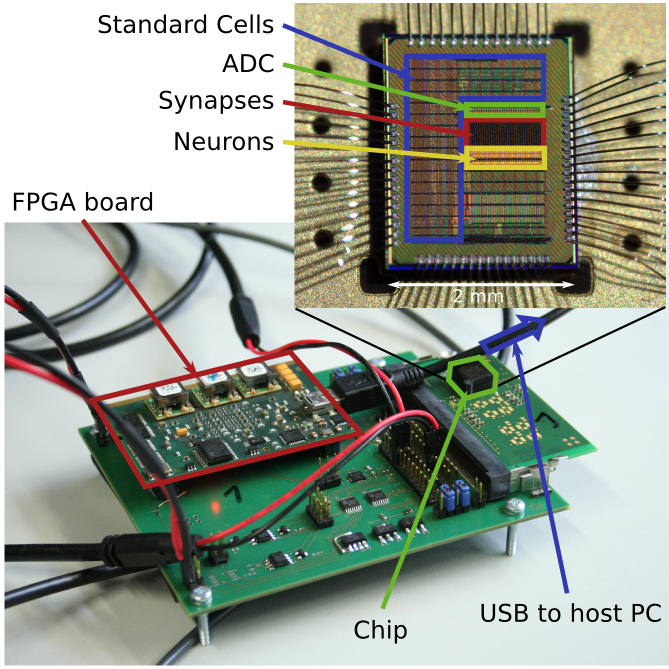
\includegraphics[width=0.4\textwidth]{pictures/Fig1.png}
    \caption{\label{fig:dlsboard} Set-Up of a \ac{HICANN-DLS} Test System (taken from~\citeauthor{PPU})}
\end{wrapfigure}
\\
Until now full compiler support does not exist for the \ac{PPU} because of its modified processor architecture, which was developed solely for neuromorphic hardware.
It offers a partly customized instruction set that is optimized for its applications.
\\
The \ac{HICANN-DLS} already is an experimental platform, which is used by several users, even though of \ac{PPU}-related challenges.
Applications like in-the-loop training or \ac{STDP} have been developed and mostly do not involve the \ac{PPU} .
Even when taking the effort of learning to code for the \ac{PPU}, users are constantly challenged by missing programming features such as creating parameterized functions.
This leads to repetitive code or difficulties when integrating calibration into experiment-related code.

Offering more tools for \ac{PPU} programs could reduce the effort of developing for the \ac{PPU}, while at the same time increasing capabilities of programs.
Besides allowing full high-level programming, compiler support could also offer tools like code optimization and debugging features.
At some point compiler support may also facilitate automatic code generation as a prerequisite for implementation of very high-level languages.
Users then could create plasticity rules in existing program environments, from where code is translated into \ac{PPU} programs.
This creates the need for optimization of \ac{PPU} code, like those built into virtually every compiler.
\\
\\
This thesis will focus on achieving aforementioned compiler support and briefly explain the process itself.
As fundamental knowledge of both, processors and compilers, is needed along the way, the second chapter will start with a very basic introduction to both topics.
This involves basic information about the \ac{PPU}, as well as the \ac{GCC}, and should explain the basic concepts to an extend which is sufficient.
Afterwards, the process of extending the compiler is explained, followed by a presentation of results as well as first test cases.
The thesis will conclude in a resume and give an outlook to future applications and development of the compiler and the \ac{PPU}.
